\documentclass{sciposter}
\usepackage{lipsum}
\usepackage{epsfig}
\usepackage{amsmath}
\usepackage{amssymb}
\usepackage{multicol}
\usepackage{listings}
\usepackage{graphicx,url}
\usepackage[spanish, spain]{babel}   
\usepackage[utf8]{inputenc}
%\usepackage{fancybullets}
\newtheorem{Def}{Definition}
\usepackage{listings}
\usepackage{xcolor}

\definecolor{lightgray}{gray}{0.95} % Color de fondo personalizado

\lstset{
  backgroundcolor=\color{lightgray},
  basicstyle=\ttfamily\small,
  keywordstyle=\color{blue},
  commentstyle=\color{gray},
  numbers=left,
  numberstyle=\tiny\color{gray},
  frame=single,
  captionpos=b
}

\title{Proyecto Integrador Nº1
\\ }
%Título do projeto

\author{Ignacio Nahuel Chantiri 69869/1}
%nome dos autores

\institute 
{Facultad de Ingeniería de la Universidad Nacional de La Plata}
%Nome e endereço da Instituição

%\date is unused by the current \maketitle



\begin{document}
%define conference poster is presented at (appears as footer)



\maketitle

%%% Begin of Multicols-Enviroment
\begin{multicols*}{2}

%%% Introduction
\section{Introducción}
El siguiente informe documenta la selección e implementación de un algoritmo de ordenamiento (en orden creciente) de vectores numéricos, a ser desarrollado en arquitectura MARIE; acompañado de un estudio de performance y una comparación de los distintos tipos de soluciones para el problema de ordenamiento.\\



\section{Consideraciones para la selección adecuada del Algoritmo}

Se tuvieron en cuenta distintos parámetros para la selección del algoritmo:

\begin{itemize}
    \item \textbf{Complejidad de implementación en MARIE:} El desarrollo de cualquier algoritmo, en general, es más complejo cuando se realiza en lenguaje ensamblador. A esto se suma que MARIE cuenta con un repertorio de instrucciones más limitado que otras arquitecturas, haciendo aún más compleja la implementación de algunos algoritmos, por ejemplo, los que hacen uso de una pila, puesto que no se dispone de instrucciones nativas para su manejo.
    
    \item \textbf{Memoria utilizada:} MARIE cuenta con una memoria de instrucciones de 4096 celdas. Aunque pueda parecer una cantidad considerable, planteese la siguiente situación:\\
    Los algoritmos más complejos, como el Quick Sort, son superadores en eficiencia mientras más largo sea el vector a ordenar.\\
    Al mismo tiempo, mientras más largo es el vector a ordenar, más espacio de memoria se ocupa no solo por el vector mismo, sino por el agrandamiento de la pila (que en cierto momento será igual de grande que el vector).\\
    Se forma entonces un dilema: \textit{Mientras más grande el vector, más eficiente el algoritmo, pero si el vector es muy grande, quizá no se pueda implementar el mismo algoritmo debido al gran espacio que ocuparía}.
    
    \item \textbf{Eficiencia:} MARIE cuenta con un solo registro (acumulador) para realizar comparaciones o aritmética. Esto significa que se requiere buscar uno de los argumentos en memoria, lo cual es ineficiente en el sentido de la cantidad de ciclos de reloj que requiere.\\
    En algunos algoritmos simples, es predecible la cantidad de accesos de memoria que se ejecutarán, permitiendo optimizarlos en ese sentido.
\end{itemize}

A continuación se desarrollan varios puntos a favor y en contra de los principales algoritmos, que llevaron a la decisión final, junto con una breve descripción de los mismos:

\subsection{Bubble Sort}
Compara dos elementos consecutivos del vector y los ordena. Repite iterativamente con los dos elementos siguientes hasta que el vector esté completamente ordenado.\\
La mayor ventaja es su facilidad de implementación. Al hacer uso de solo dos punteros, no requiere prácticamente espacio de memoria extra para una pila. Además, para ordenar vectores cortos, se desempeña de manera similar que otros algoritmos considerados más eficientes.

\subsection{Selection Sort}
Este algoritmo busca el menor elemento y lo ubica al comienzo, iterativamente.\\
Otro algoritmo de fácil implementación y de velocidad (su desventaja) similar al Bubble Sort. Tampoco ocupa una cantidad considerable de memoria.

\subsection{Insertion Sort}
Inserta cada nuevo elemento en la posición correcta dentro de una parte del vector ya ordenada.\\
Su implementación es relativamente más dificultosa que los algoritmos anteriores, aunque no muy compleja. No ocupa una cantidad considerable de memoria. Se descartó por no ofrecer una velocidad mayor que otras opciones más simples.

\subsection{Merge Sort}
Divide el vector a la mitad, recursivamente (problema).
Requiere un espacio extra igual al vector original, haciéndolo mala opción para vectores grandes.\\
Utiliza recursividad, lo que torna dificultosa su implementación.
Las ventajas podrían compensar estas desventajas, pues es muy eficiente (en velocidad) aún con vectores muy grandes.

\subsection{Quick Sort}
Toma un pivote, y divide entre números mayores o menores a él, repitiendo de manera recursiva para cada sub-vector resultante.\\
Otro algoritmo recursivo muy eficiente para vectores largos, parecido al Merge Sort, pero que también requiere mucho espacio y utilización de pila.\\

\section{Algoritmo elegido: Bubble Sort}
Se decidió implementar el algoritmo \textbf{Bubble Sort}.
Como el objetivo principal es ordenar un vector de 7 elementos, no se aprovecha la capacidad de los algoritmos más complejos de ordenar vectores largos eficientemente.
En la siguiente tabla se compara el algoritmo elegido junto con uno más complejo:

\begin{center}
\begin{tabular}{|c|c|c|}
\hline
\textbf{Caso} & \textbf{Bubble Sort} & \textbf{Quick Sort} \\
\hline
Mejor         & $O(n)$              & $O(n \log_2 n)$     \\
\hline
Promedio      & $O(n^2)$            & $O(n \log_2 n)$     \\
\hline
Peor          & $O(n^2)$            & $O(n^2)$            \\
\hline
\multicolumn{3}{|c|}{\textbf{Operaciones estimadas para n=7 )}} \\
\hline
\textbf{Caso} & \textbf{Bubble Sort} & \textbf{Quick Sort} \\
\hline
Mejor         & $7$                  & $7 \cdot \log_2 7 \approx 19.65$ \\
\hline
Promedio      & $49$                 & $7 \cdot \log_2 7 \approx 19.65$ \\
\hline
Peor          & $49$                 & $49$                 \\
\hline
\end{tabular}
\end{center} 

En la última sección de la tabla se observan los resultados para el vector de 7 elementos que se requiere ordenar.\\
Para el mejor caso de cada uno, el Bubble Sort realiza menos de la mitad de operaciones que el Quick Sort.\\
Para el caso promedio, el Quick Sort realiza menos de la mitad de operaciones que el Bubble Sort.\\
Para el peor caso, realizan la mismas operaciones.\\

Es importante tener en cuenta que el peor caso para cada algoritmo se da bajo distintas condiciones: para el Quick Sort, el peor caso depende de la correcta elección del pivote, y no necesariamente de que tan ordenado está el vector orignalmente, mientras que para el Bubble Sort el vector invertido es el peor caso; por lo que estas conclusiones son estimadas.\\

En resumen, existe un comportamiento muy parecido entre ambos algoritmos para el caso n = 7, por lo que no vale la pena implementar un algoritmo más complejo para obtener casi el mismo resultado.\\
Si nos valiésemos más por lo que sucede en el caso promedio, quizá Quick Sort sea la mejor implementación. Pero para el caso requerido, en el que hay que ordenar un vector ordenado, uno invertido, y uno random, el resultado promedio es el similar independientemente del algoritmo.\\

Por último, el desarrollo en lenguaje ensamblador fué muy rápido para el Bubble Sort en comparación con el del Quick Sort.\\

\section{Desarrolo del código en detalle}

\subsection{Esquema general}

\begin{figure}[H]
    \centering
    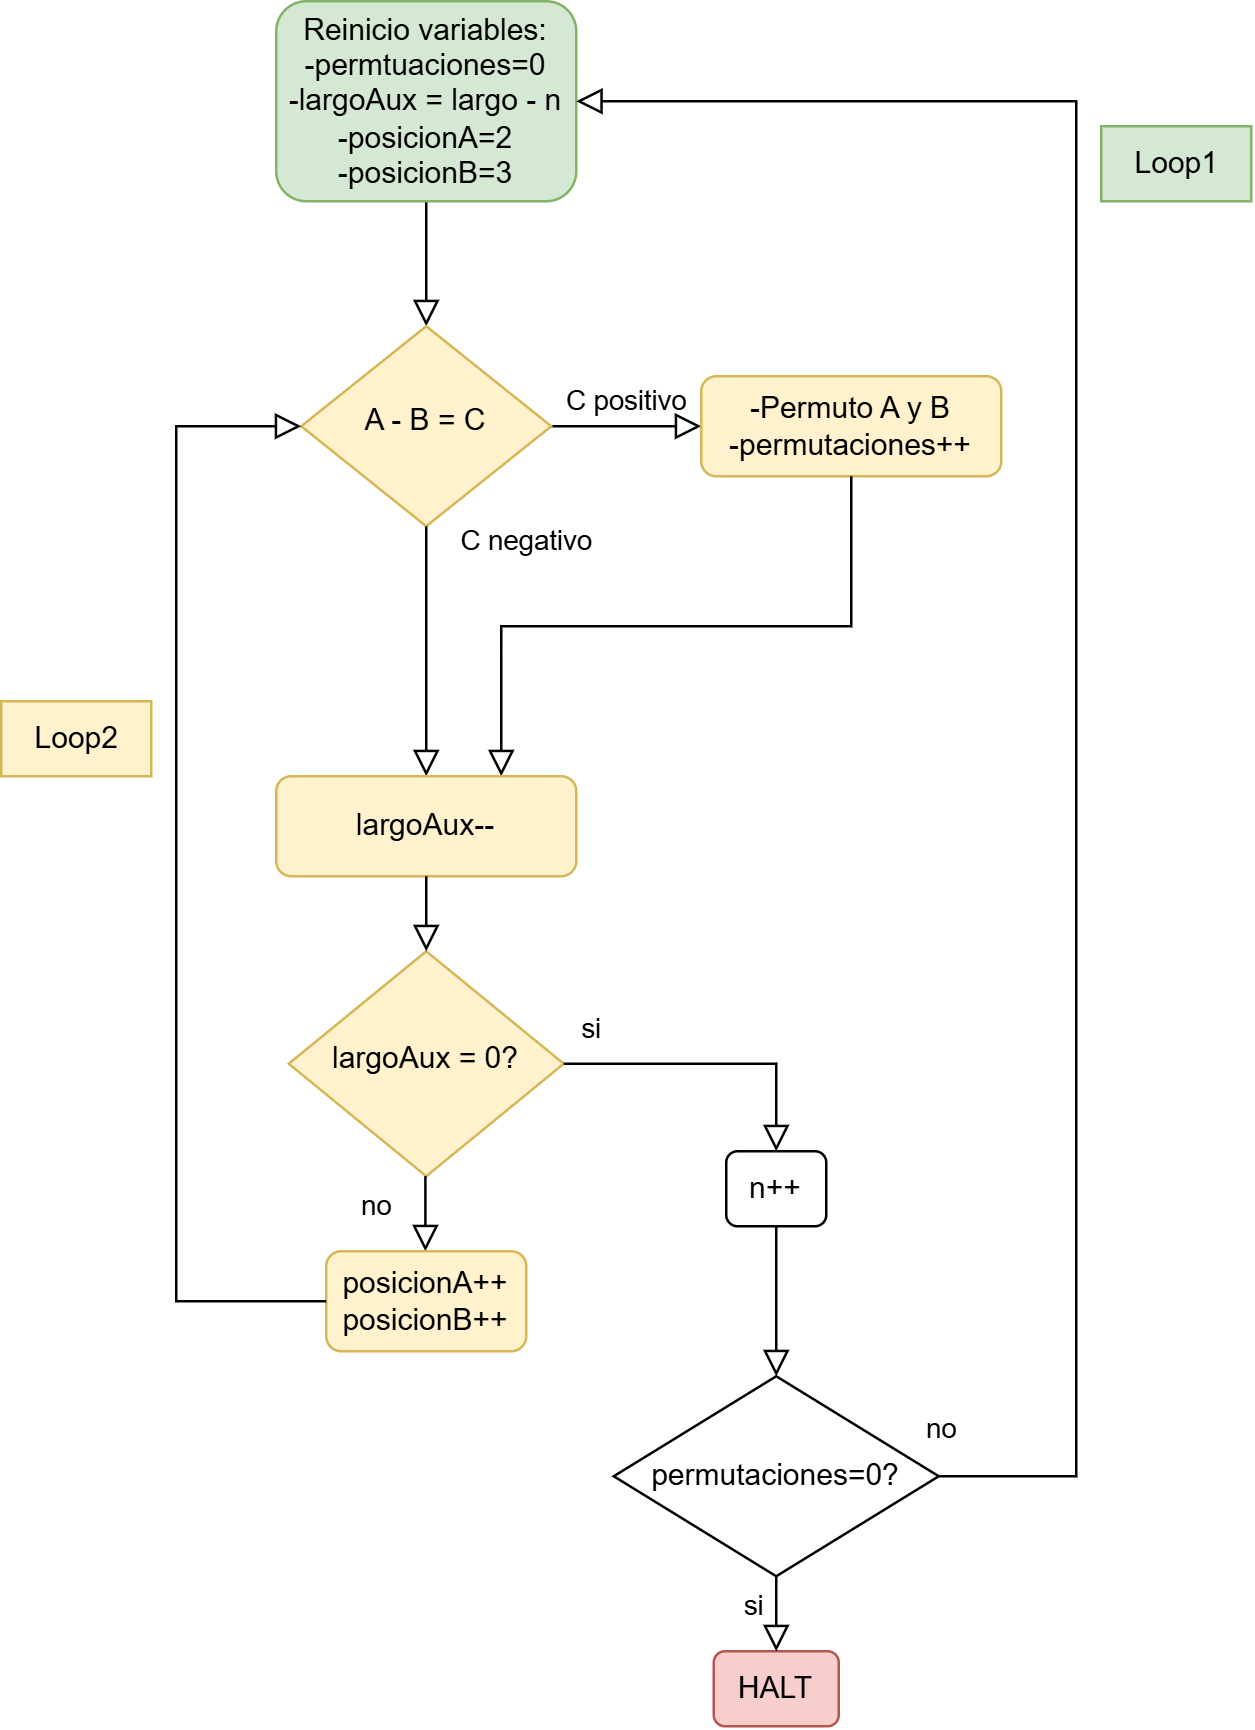
\includegraphics[width=0.7\linewidth]{Diagrama Bubble Sort.drawio.png}
    \caption{Esquema general del código implementado para el Bubble Sort}
    \label{fig:enter-label}
\end{figure}

\subsection{Pseudo-código}

La implementación se reduce al siguiente pseudo-código:

\begin{lstlisting}
largo = largo del vector
n = 1

Loop1{ 
     permutaciones = 0
     largoAux = largo - n
     punteroA = 0
     punteroB = 0

     Loop2{ 
          Comparo A con B
          Permuto si es necesario
          permutaciones ++
          punteroA ++
          punteroB ++
          largoAux --
          if largoAux = 0, salgo de Loop2
          }
    n ++
    if permutaciones = 0, salgo de Loop1
     }
Halt
    
\end{lstlisting}

\subsection{Explicación general}

El código es relativamente simple:
Los elementos en \underline{\textbf{negrita}} (A y B respectivamente) son comparados, y si es necesario, permutados. La comparación se explica en detalle en la \textbf{sección 4.2}.

\begin{center}
    \underline{\textbf{3}}, \underline{\textbf{2}}, 1, 0, -1, -2, -3
\end{center}

Luego se aumentan los punteros de A y B, seleccionando los dos elementos siguientes, y se repite la operación sucesivamente hasta recorrer el vector completo.\\
La variable largoAux hace de flag para detectar si ya se recorrió el vector completo.
\begin{center}
    2, \underline{\textbf{3}}, \underline{\textbf{1}}, 0, -1, -2, -3
\end{center}
\begin{center}
    2, 1, \underline{\textbf{3}}, \underline{\textbf{0}}, -1, -2, -3
\end{center}
\begin{center}
    ...
\end{center}
\begin{center}
    2, 1, 0, -1, -2, -3, \textbf{3}
\end{center}

Cuando se detecta que el vector fue recorrido en su totalidad, se verifica si hubo alguna permutación.\\
Si la hubo, no sabemos con certeza si el vector está ordenado, por lo que recorremos nuevamente (esta vez recorremos hasta el índice \textit{largoAux - n}, donde \textit{n} indica la cantidad de veces que se recorrió el vector. Esto se debe a que en cada recorrida, el último elemento ya está en su lugar final, y no hace falta compararlo). Se repite sucesivamente hasta que no haya permutaciones.\\
Cuando no se detecta ninguna permutación, el algoritmo finaliza y el vector se halla en su posición orginal, ordenado.\\

\subsection{Comparación}

La comparación se realiza mediante la resta A - B = C.\\
Observando el signo de C, se puede determinar si A o B es mayor, sin importar el signo de los elementos, tal que:\\

\begin{center}
    Si $C \geq 0$ , \textbf{NO} se permuta A con B
\end{center}
\begin{center}
    Si $C < 0$, se permuta A con B
\end{center}
La ventaja de este método es su extrema simplicidad, ya que con una misma operación es posible comparar elementos de cualquier signo, aún si los elementos son iguales, o si alguno (o ambos) son cero.\\
Sin embargo, se debe tener en cuenta que MARIE permite representar números de hasta 16 bits en Ca2, por lo que habrá ciertos casos en el que se genere overflow.\\
Por ejemplo, suponer el caso en que se comparan los siguientes números:

\begin{center}
    \textbf{A} = 32.767 (máximo numero en Ca2 que representa MARIE)
\end{center}

\begin{center}
    \textbf{B} = -1
\end{center}

La comparación A - B dará como resultado 32.767, que no es representable con 16 bits en Ca2, provocando un overflow. La misma situación sucede siempre que \( \left| A - B \right| > 32.767 \)
, por lo que ningún par de elementos del vector debería exceder esa condición para asegurar el correcto funcinoamiento del algoritmo.\\
El código implementado no considera estas situaciones. MARIE tampoco cuenta con un registro de estados para verificar si sucedió un overflow, aunque el simulador web sí.

\section{Especificaciones}
\subsection{Memoria utlizada}
El código completo, considerando memoria de programa y datos (sin incluir el espacio ocupado por el vector, la celda que indica su largo, y el jump que llama a la función) ocupa \textbf{48} direcciones de memoria (39 de programa y 9 de datos) de las 4096 disponibles, esto es \textbf{el 1.17\%  del total de la memoria}, o expresado en bytes, \textbf{96 bytes}.\\

La memoria utilizada se midió mediante el recuento manual de las líneas del programa.\\

\subsection{Performance}
Se detallan la candidad de instrucciones ejecutadas para tres casos distintos, según el grado de orden del vector:

\begin{itemize}
    \item \textbf{Vector ordenado (mejor caso): 106 instrucciones, 713 ciclos de reloj} 
    \item \textbf{Vector invertido (peor caso): 527 instrucciones, 3739
ciclos de reloj}
    \item \textbf{Vector desordenado (caso promedio): 477 instrucciones, 3299 ciclos de reloj}
\end{itemize}

Para la medición de ciclos e instrucciones se utilizó la versión modificada del simulador web de MARIE que provee la cátedra.

\section{Conclusiones}

El trabajo de investigación sobre los distintos algoritmos de ordenamiento proporciona no solo un entendimiento sobre las capacidades de la arquitectura utilizada, sino también una apreciación por la complejidad de implementar algoritmos en sistemas con recursos limitados.\\

Al intentar implementar varios de los algoritmos, se evidenciaron las características de MARIE como arquitectura, que, usualmente, favorecen soluciones más simples. \\

Las especificaciones del proyecto, que implicaban la ordenación de tres vectores específicos, destacan la importancia de un enfoque con mayor criterio: el algoritmo más eficiente no siempre es el mejor cuando se considera el contexto real del hardware y las restricciones. La eficiencia no solo se mide en términos de tiempo de ejecución, sino también en el uso de los recursos disponibles, como la memoria y el acceso a registros.

\end{multicols*}

\end{document}